%!TEX root = ../report.tex
\chapter{Path planning} % (fold)
\label{chap:path_planning}

In this chapter, the path planning for the robot is presented.
The first section deals with the path planning problem found in our case. Then, the constrained planning along with the assumptions made are presented. Follows the collision avoidance strategy. In the end, the implementation, the experimental results and the conclusions of this chapter are presented.

\section{Path planning in keep object in sight} % (fold)
\label{sec:path_planning_in_keep_object_in_sight}
The problem treated is keep an object in sight. 
Due to the nature of the low speed of the object to be tracked, the movement increments that the robot is going to achieve are in the order of centimeters. 
This, with the low colliding objects in the work cell where the experiment is carried out, gives as a result to focus in the main problem of keeping an object in sight: the constrained planning.
% section path_planning_in_keep_object_in_view (end)

\section{Constrained planning} % (fold)
\label{sec:constrained_planning}
From now the assumption of that the object is being located is taken. 
Despite the object tracked is referenced to the camera's frame, in the name of clarity, lets assume that the object tracked is in the world's reference frame. 
For now, a point in the space is located along with the robot.
The goal is find a robot configuration that always allows to keep the camera in direction to the tracked object.
Thus, the problem is reduced to find a camera's pose that is looking to the object.
This is not trivial due to there are infinite solutions as is going to be shown now. \\

The pose to be found is composed of a vector that defines the position in the spaces, this is the $x$, $y$ and $z$ coordinates, and the orientation matrix what, in order to clarify the concept, lets assume that this matrix is expressed in the Euler Angles with RPY. So the unknowns of the problem is expressed in a vector of 6 components being this:
	\begin{equation}
	\label{eq:pose_cartesian_coordinates}
		Pose = [x,y,z,R,P,Y]
	\end{equation}

\subsection{X, Y and Z coordinates} % (fold)
\label{sub:x_y_and_z_coordinates}
To reduce the degrees of freedom of the problem two assumptions are taken:
\begin{enumerate}
	\item The robot's base is located in the World reference frame.
	\item The camera will be at a fixed distance from the object.
\end{enumerate}
The explanation for this assumption will be explained later. While the reason for the second is to reduce the problem to a smaller set of solutions. Now, the possible poses can be expressed as an non-solid sphere around the tracked object.
Due to our problem, an always desired position is the one that in which the camera is contained in the plane formed by the robot's z base axis and the tracked point. This reduce the problem from an non-solid sphere to a circle's perimeter as result from the cut from the plane to the sphere.
Due to the robot is contained in this pane, makes more probable for the robot to find a future possible configuration.\\

So based in our assumption of fixed distance, a better way to express the pose is the one that includes the distance to the object as a variable.  
This is, we have to define a distance that allows to keep the tracked object enough far to have its whole shape and enough short to being able to focus the object.
For this reason, and this is only valid when the robot's base is centered in the World's reference frame, polar coordinates are used to express the pose vector from \ref{eq:pose_cartesian_coordinates}. So now this is:
	\begin{equation}
	\label{eq:pose_polar_coorinates}
		Pose = [r,\alpha,z,R,P,Y]
	\end{equation}
So transforming the 3D point of the tracked object to polar coordinates we can obtain the desired pose angle $\alpha$ and the radius $r$. 
The angle is the same based on the first assumption and because we want the camera to be in the plane formed by the robot's z base axis and the tracked point. 
The radius can be calculated as the actual $r_object$ minus the desired distance to the object. Is minus because we want it in the direction of the robot's base. 
So the camera's pose is now defined as:
	\begin{equation}
	\label{eq:cameras_pose_noRPY_noZ}
		Pose_{camera} = [r_{object},\alpha_{object},z,R,P,Y]
	\end{equation}
The height keeps being an unknown but and, due to the next position of the object is unknown, not predictions about the height can be made. 
For this reason the camera's height is assumed to be the same as the tracked object. This assumption included in the equation \ref{eq:cameras_pose_noRPY_noZ} gives:
	\begin{equation}
		\label{eq:cameras_pose_noRPY}
		Pose_{camera} = [r_{object},\alpha_{object},z_{object},R,P,Y]
	\end{equation}
% subsection x_y_and_z_coordinates (end)
\subsection{R, P and Y angles} % (fold)
\label{sub:r_p_and_y_angles}
Knowing that the camera's reference frame will be that one contained in the plane expressed previously, its Z axis must look to the point. 
Assuming that the X and Y axis are parallel to the robot's base frame the angles can be obtained easily.
This assumption is consistent with the same idea applied in the obtainment of the height. 
The future state of the object is unknown and due to the robustness of the system is searched, the camera would look directly to the object.\\

This implies that the camera's Z axis must look to the point, so the roll (r) should be the transformation from the robot's base to the camera + the angle from the polar coordinates calculated previously.
Regarding the the pitch (P) and the yaw (Y), is more likely to find a valid state solution if these are parallel to the robot's base reference frame. 
The camera can be put in another alignment than the base which would include an offset in R,P and/or Y, but supposing the axis are aligned, the final camera's pose is:
	\begin{equation}
		\label{eq:cameras_pose}
		Pose_{camera} = [r_{object},\alpha_{object},z_{object},\alpha_{object},0,0]
	\end{equation}
% subsection r_p_and_y_angles (end)
Taking some assumptions the camera's pose has been reduced from infinite to one single solution. Thus, the problem now is check if this pose is reachable by the robot.\\

This is made applying inverse kinematics. The IK should give a vector of possible solutions from which only one should be chosen. This is the one that is energetically better than the rest. This means, the one who moves less joints.

% section constrained_planning (end)

\section{Path optimization} % (fold)
\label{sec:path_optimization}
Due to the speed at which the points are received, the incremental movements of the robot tend to be small. Thus, there is few room for path optimization. However given two Q's an interpolation between them has been made.\\

A natural cubic interpolation as shown in the figure \ref{fig:cubic interpolation}, is made. The number of interpolated steps can be controlled affecting to the robot so, a higher number means more smoothness but more path time and less speed, and vice versa.

\begin{figure}[!hb]
	\centering
	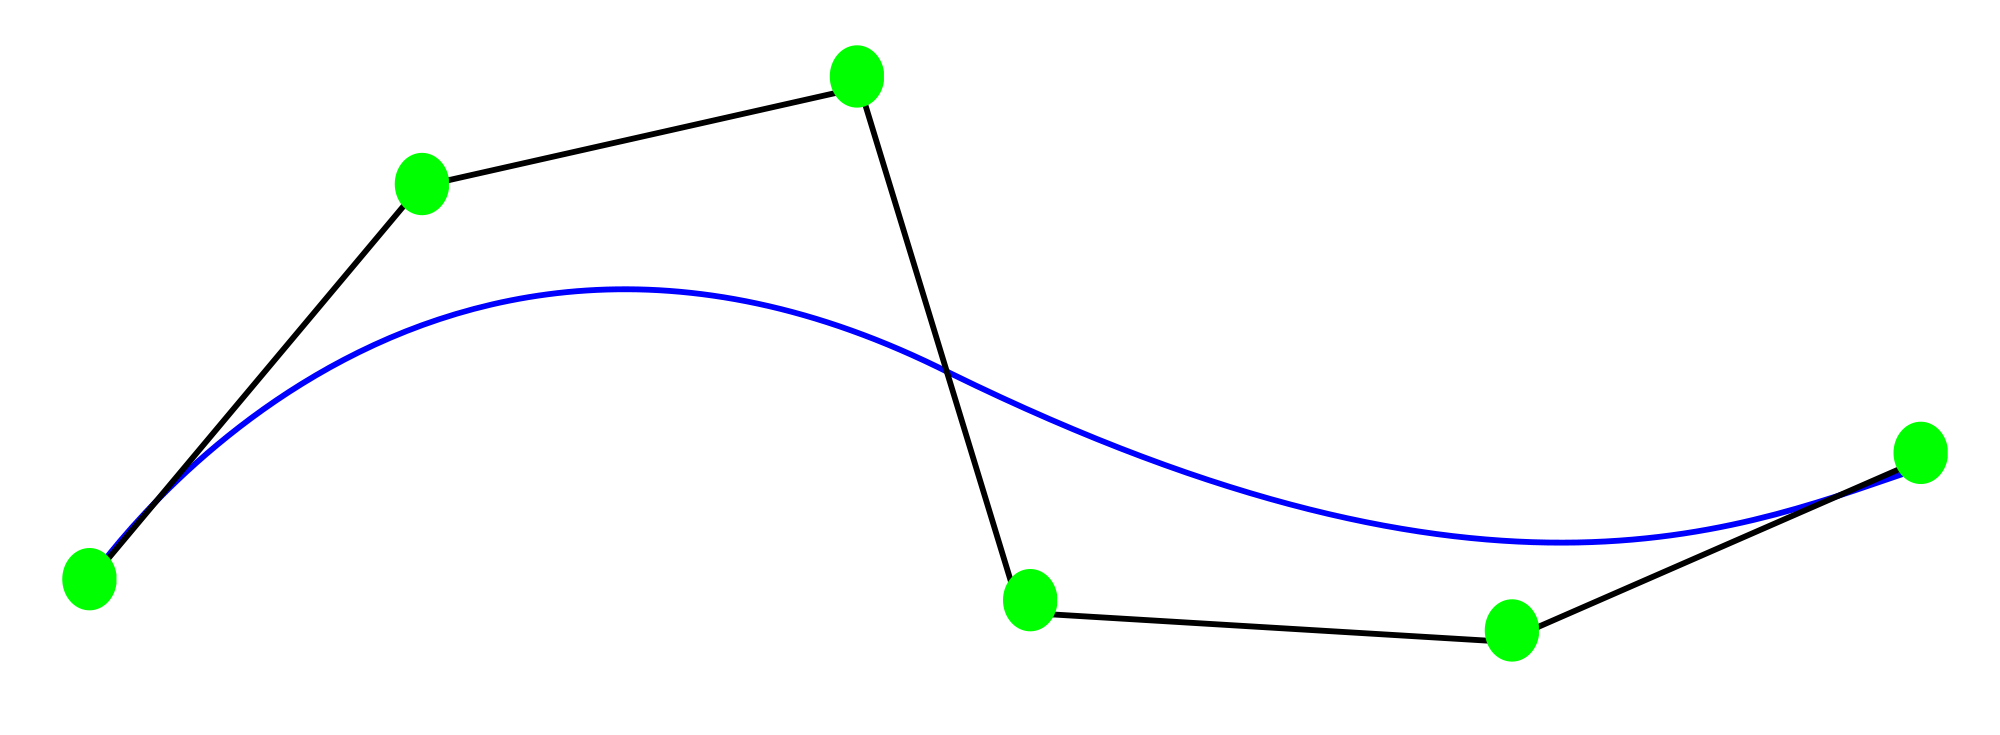
\includegraphics[width=0.8\textwidth]{figures/cubic_interpolation}
	\caption{Cubic interpolation}
	\label{fig:cubic interpolation}
\end{figure}
% section path_optimization (end)

\section{Collision avoidance} % (fold)
\label{sec:collision_avoidance}
For each interpolated Q, a single query planner with in the robot's collision free space, is checked. If a future collision is detected the Rapid-exploring Random Tree RRT in its variance RRT-Connect \cite{RRTConnect} is used.\\

This method is an online method to generate random configurations in the collision free space.
The algorithm used is presented in the listing \ref{lis:rrt_connect_planner} and it defines how from a $q_{init}$ to a $q_{goal}$ $\in$ \ $C_{free}$, a random configuration tree is expanded and connected  until the init reach the goal. The RRT-Connect (see figure \ref{fig:rrt_connect}) is not tunned by a parameter but the random Q's generation is defined by a defined distance and the used metric to defined that distance.

\begin{lstlisting}[frame=tb, mathescape=true, xleftmargin=.28\textwidth, xrightmargin=.28\textwidth,caption=RRT-Connect Algorithm, label=lis:rrt_connect_planner]
$\textbf{CONNECT}$($\Gamma$, $q$)
 1  repeat 
 2  S $\leftarrow$ EXTEND($\Gamma$,$q$);
 3  until not (S=Advanced)
 4  Return S;
\end{lstlisting}
\lstset{}

\begin{lstlisting}[frame=tb, mathescape=true,xleftmargin=.13\textwidth, xrightmargin=.13\textwidth]
$\textbf{RRT CONNECT PLANNER}$($q_{init}$,$q_{goal}$)
 1  $\Gamma_a$.init($q_{init}$);$\Gamma_b$.init($q_{goal}$);
 2  for k = 1 to K do
 3    q rand $\leftarrow$ RANDOM CONFIG();
 4      if not (EXTEND($\Gamma_a$,$q_{rand}$)=Trapped) then
 5        if (CONNECT($\Gamma_b$,$q_{new}$)=Reached) then
 6        Return PATH($\Gamma_a$,$\Gamma_b$);
 7    SWAP($\Gamma_a$,$\Gamma_b$);
 8  Return Failure
\end{lstlisting}

\begin{figure}[!ht]
	\centering
	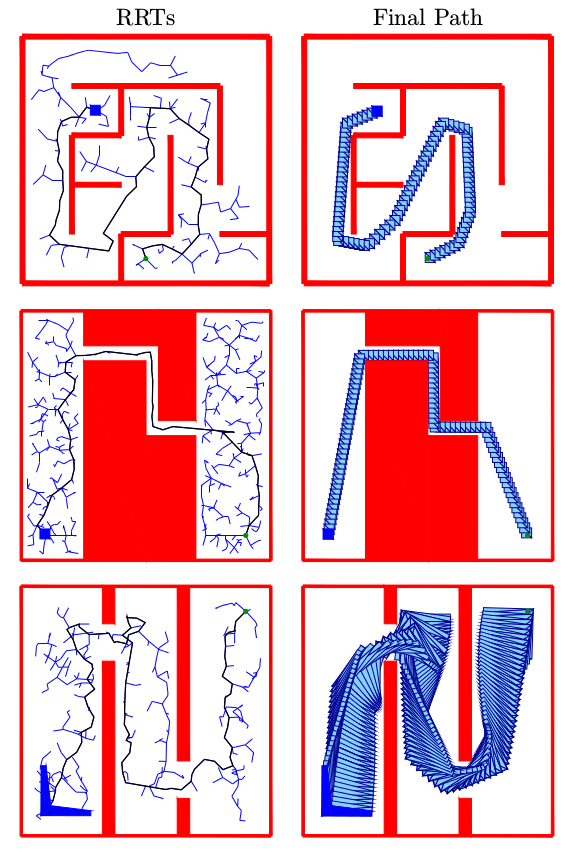
\includegraphics[width=0.4\textwidth]{figures/rrt_connect}
	\caption{RRT-Connect Example}
	\label{fig:rrt_connect}
\end{figure}

% section collision_avoidance (end)

\section{Implementation} % (fold)
\label{sec:implementation}
\begin{figure}[!hb]
	\centering
	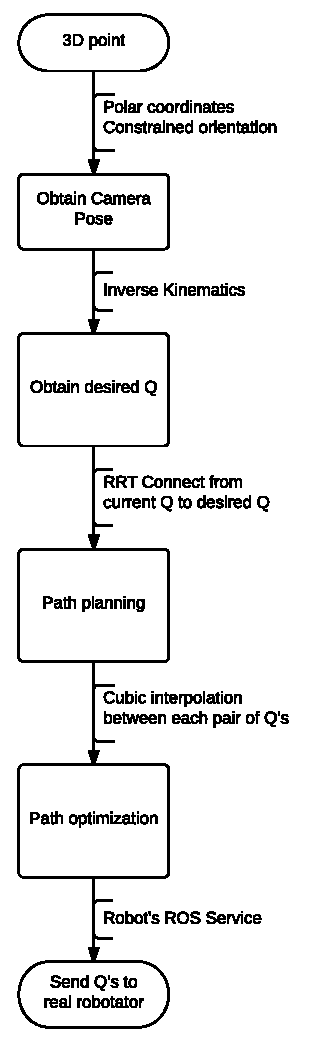
\includegraphics[height=16cm]{figures/path_planning_flowchart}
	\caption{Flowchart of the path planning method}
	\label{fig:path_planning_flowchart}
\end{figure}
% section implementation (end)

\section{Experimental results} % (fold)
\label{sec:experimental_results}

% section experimental_results (end)

\section{Conclusions} % (fold)
\label{sec:conclusions}

% section conclusions (end)

% chapter path_planning (end)